      
               
                \begin{ledgroupsized}[r]{120mm}
                \footnotesize 
                \pstart             
                \noindent\textbf{\"{U}berlieferung:}   
                \pend
                \end{ledgroupsized}
            
              
                            \begin{ledgroupsized}[r]{114mm}
                            \footnotesize 
                            \pstart \parindent -6mm
                            \makebox[6mm][l]{\textit{L}}Reinschrift mit Verbesserungen: LH XXXVIII Bl. 25. 1 Bl. 4\textsuperscript{o}. 1 S. auf Bl.~25~r\textsuperscript{o} und 3~Z. auf Bl.~25~v\textsuperscript{o}. Fragment eines Wasserzeichens.
\\ Cc 2, Nr. 1192 C 
\pend
                            \end{ledgroupsized}
                %\normalsize
%                \vspace*{4mm}
%                \begin{ledgroup}
%                \footnotesize 
%                \pstart
%            \noindent\footnotesize{\textbf{Datierungsgr\"{u}nde}: Der Text steht inhaltlich in engem  Zusammenhang mit N. ??
%%LH035_10_09_001-4_intro.tex = Regle pour calculer la force d'une machine        
%. Zudem könnten die Wasserzeichen identisch sein. Daher wird die Datierung von N. ??
%%LH035_10_09_001-4_intro.tex = Regle pour calculer la force d'une machine  
%übernommen.}
%                \pend
%                \end{ledgroup}
            
                \vspace*{6mm}
               \pstart 
\normalsize
\noindent
[25~r\textsuperscript{o}]
\pend
\pstart
\centering
\noindent
\edtext{Preparation}{\lemma{}\Bfootnote{\textit{(1)}\ Construction \textit{(2)}\ Preparation \textit{L}}}
\pend
\count\Bfootins=1000
\count\Cfootins=1000
\pstart \noindent \selectlanguage{french}Dans le Cercle \textit{ABCD}, soit mobile la roue Antisoscele \textit{EFGH} charg\'{e}e de 4 poids\protect\index{Sachverzeichnis}{roue antisoscele}\protect\index{Sachverzeichnis}{machine}                    
  \'{e}gaux \textit{E}, \textit{F}, \textit{G}, \textit{H}. \pend 
  \pstart Des points \textit{E}, \textit{F}, soyent menez les sinus  droits des angles d'inclination donnez, \textit{ANE}, et \textit{FNC}, s\c{c}avoir \textit{EI}, et \textit{FK}. \pend 
  \pstart  Mettons la roue\protect\index{Sachverzeichnis}{roue} dans un \edtext{autre estat}{\lemma{un}\Bfootnote{\textit{(1)}\ estat ou angle \textit{(2)}\ autre estat \textit{L}}}  d'inclination\protect\index{Sachverzeichnis}{inclination}, s\c{c}avoir dans l'estat \textit{LOPQ},  et menons de m\^{e}me les sinus droits, \textit{LM}, et \textit{OR}. \pend 
\pstart \vspace{0.8em} 
\begin{center}%
\textso{Theoreme}:%
\edlabel{LH038_025_1a}%
\edtext{}{{\xxref{LH038_025_1a}{LH038_025_1b}}{\lemma{Theoreme:}\Bfootnote{\textit{(1)}\ La Machine dans l'Estat \textit{EFGH}, est \`{a} la Machine \textit{(2)}\ La force [...] Machine \textit{L}}}}
\end{center}
\pend 
\pstart  
\noindent%
La force du commencement de la Machine\protect\index{Sachverzeichnis}{machine} quand elle commence son mouuement dans l'Estat \textit{EFGH}, est \`{a} la force du commencement de la Machine%
\edlabel{LH038_025_1b} quand elle commence dans l'Estat [\textit{LOPQ}]\edtext{}{\Bfootnote{\textit{LFGQ}\textit{\ L \"{a}ndert Hrsg.} }}, comme la droite \textit{IK} est \`{a} la droite \textit{MR}. Par consequent si la roue est \`{a} 8 dents \textit{ESFTGVHX},
dont \textit{EN}, \textit{FN}, \textit{VN},
\edtext{\textit{XN} \'{e}gales,}{\lemma{\textit{XN}}\Bfootnote{\textit{(1)}\ \'{e}gaux, item \textit{(2)}\ \'{e}gales, \textit{L}}}
et si \textit{SN}, \textit{TN}, \textit{GN}, \textit{HN}, et \textit{EG}, \textit{FH}, droites,
se coupent \`{a} angles droits aussi bien que \textit{SV}, \textit{TX},
\edtext{autres droites, et toutes les dents\protect\index{Sachverzeichnis}{dent}}{\lemma{autres droites,}\Bfootnote{\textit{(1)}\ et les points \textit{E}, \textit{S}, \textit{T}, \textit{V}, \textit{G} \textit{(2)}\ et toutes les dents \textit{L}}}
charg\'{e}es de poids \`{a} leurs
\edtext{extremitez, et les poids}{\lemma{extremitez,}\Bfootnote{\textit{(1)}\ je dis que \textit{(2)}\ et les poids \textit{L}}}
\textit{E}, \textit{F}, \textit{G}, \textit{H}, \'{e}gaux entre eux, sont aux poids \textit{S}, \textit{T}, \textit{V}, \textit{X},
aussi \'{e}gaux entre eux en raison reciproque des lignes \textit{IK}, \textit{MR}, c'est \`{a} dire, comme \textit{MR} \`{a} \textit{IK},
la roue sera en equilibre\protect\index{Sachverzeichnis}{equilibre}.
\pend
%\vspace{1mm}
\pstart \vspace{0.8em}
 \begin{center} \textso{Probleme} \end{center} \pend 
\pstart 
\noindent \textso{Trouver la situation, la plus avantageuse, pour  le commencement de la Machine.} \pend 
\pstart  Prenez l'arc \textit{AL} de 45 degrez, c'est \`{a} dire qui  soit la moiti\'{e} du Quart de Cercle \textit{ALB}, et menez la  roue \`{a} l'estat \textit{LOPQ}. Je dis que cet estat  sera le plus avantageux, c'est \`{a} dire qu'elle y commencera  avec plus de forces que dans aucun autre. \pend 
%\vspace*{8mm}
\pstart
\centering
 \hspace{0mm} 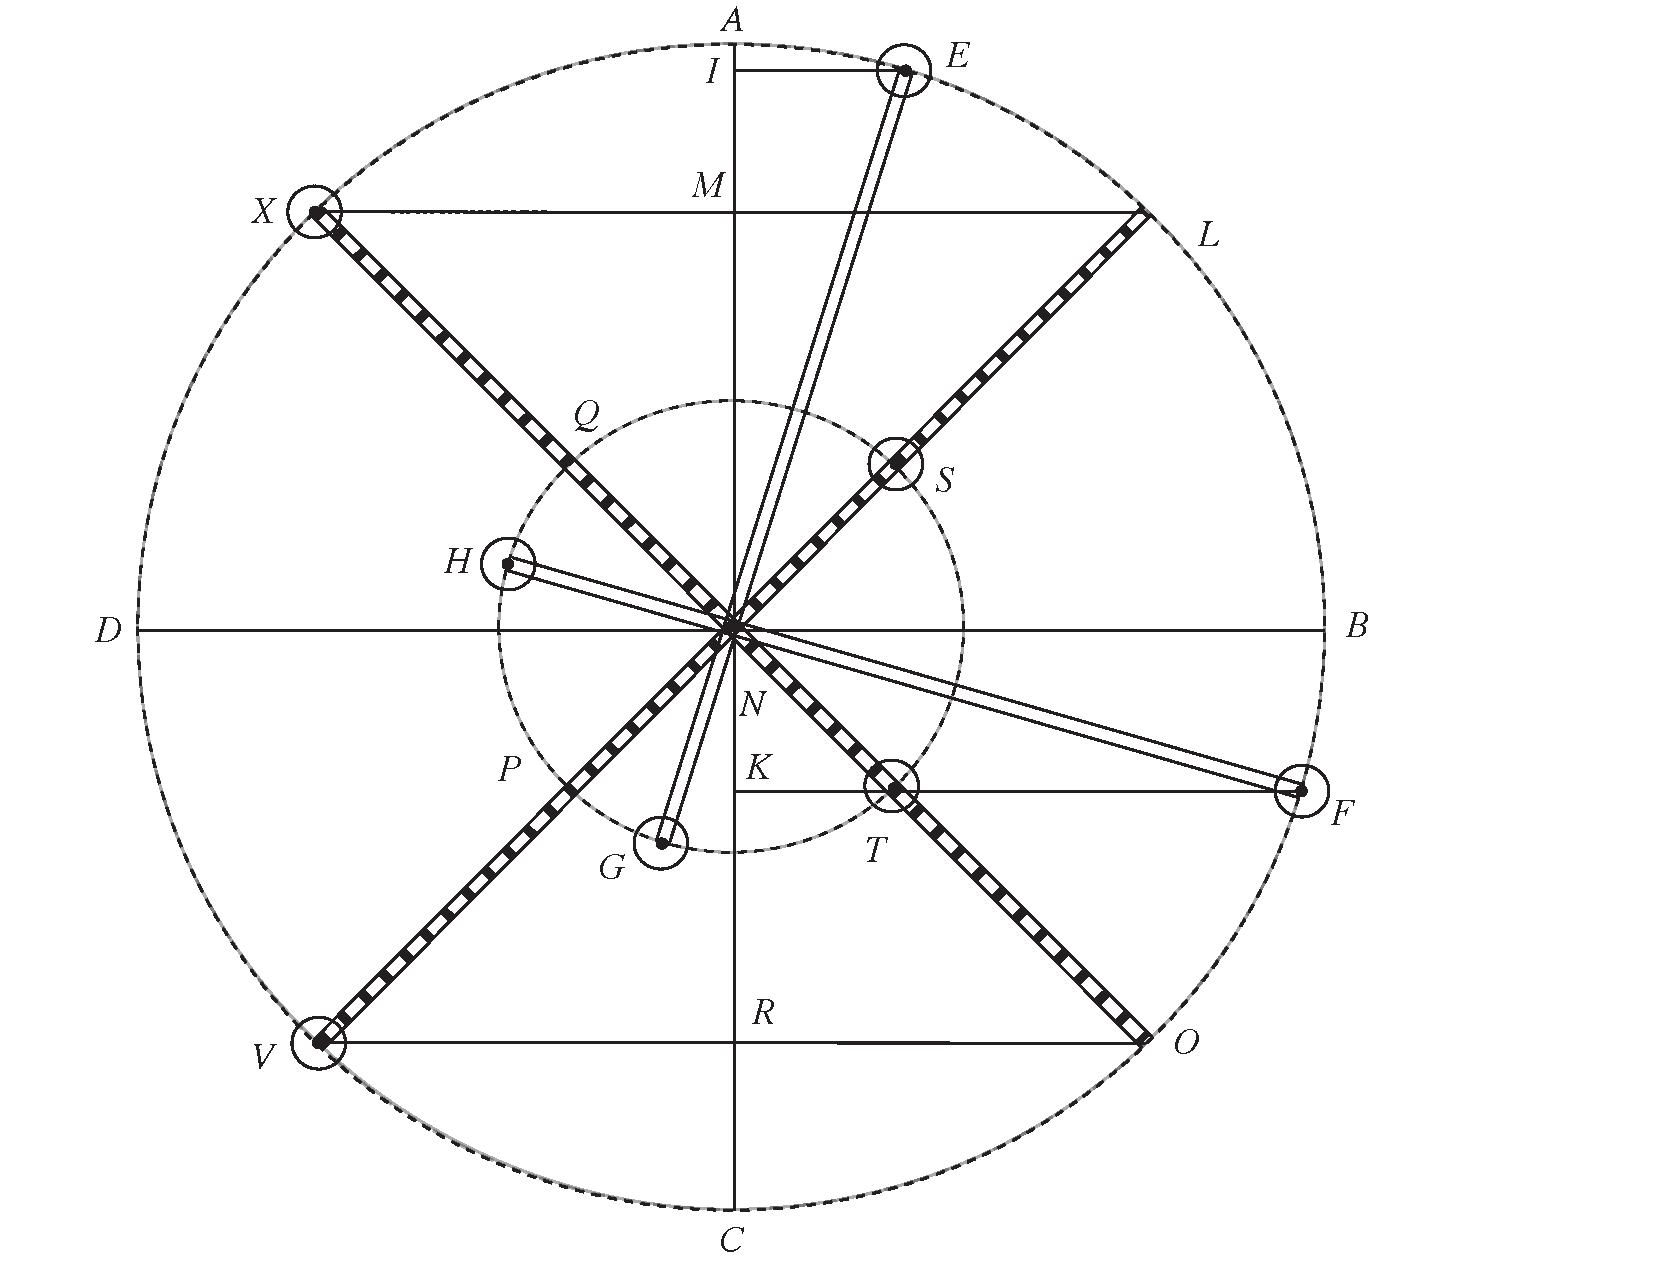
\includegraphics[width=0.9\textwidth]{images/25rx1a.pdf}
\begin{center} [\textit{Fig. 1}]
 \end{center}
\pend
\vspace{1.5em}
%\pstart \vspace{1em}
% \begin{center} \textso{Probleme} \end{center} \pend 
%\pstart 
%\noindent \textso{Trouver la situation, la plus avantageuse, pour  le commencement de la Machine.} \pend 
%\pstart  Prenez l'arc \textit{AL} de 45 degrez, c'est \`{a} dire qui  soit la moiti\'{e} du Quart de Cercle \textit{ALB}, et menez la  roue \`{a} l'estat \textit{LOPQ}. Je dis que cet estat  sera le plus avantageux, c'est \`{a} dire qu'elle y commencera  avec plus de forces que dans aucun autre. \pend 
\pstart  \centering \setline{1}Corollaire.
\pend 
%\vspace{0.5em}
\pstart \noindent Il \setline{2}s'ensuit que cette situation \edtext{du commencement}{\lemma{}\Bfootnote{du commencement \textit{erg.} \textit{L}\ }} sera la plus avantageuse non seulement  pour le commencement de la Machine\protect\index{Sachverzeichnis}{machine}, mais aussi pour sa  continuation, et par consequent, absolument. Parce que toute  la difficult\'{e} n'est que dans le commencement, et si elle peut commencer malgr\'{e} les \textso{forces permanentes} (s'il m'est permis de parler ainsi) \edtext{ou tousjours \'{e}gales,}{\lemma{}\Bfootnote{ou tousjours \'{e}gales, \textit{erg.} \textit{L}\ }} dont on la charge; \edtext{}{\lemma{}\Bfootnote{charge;  \textbar\ et \textit{gestr.}\ \textbar\ elle \textit{L}}} elle pourra continuer, \`{a} cause des forces qu'elle gagne par l'acceleration. 
\pend 
\vspace{1em}
\pstart   \centering Scholie.
\pend 
\pstart \noindent Quoyque cette Regle\protect\index{Sachverzeichnis}{regle} soit tres ais\'{e}e, la demonstration pourtant en est  tres difficile; et elle a est\'{e} trouu\'{e}e ny par hazard, ny par conjectures, ny par l'essay, mais par l'Analyse Geometrique.\protect\index{Sachverzeichnis}{analyse géométrique} Au reste la force\selectlanguage{latin} [25 v\textsuperscript{o}] \selectlanguage{french}de l'Estat \textit{ABCD} qui est le plus foible est \edtext{celle}{\lemma{}\Bfootnote{celle\textit{ erg.} \textit{L}}} \`{a} l'Estat \textit{LOPQ} qui est le plus avantageux, comme 7 \`{a} 10,  \`{a} peu pr\`{e}s.\selectlanguage{latin} 
\pend
\count\Bfootins=1500
\count\Cfootins=1500


 
 


 


 


 



 


 


 


 


 


 


 


 


 


 

